\begin{figure*}[hb]
  \centering

  \begin{subfigure}[t]{0.475\tw}\centering
    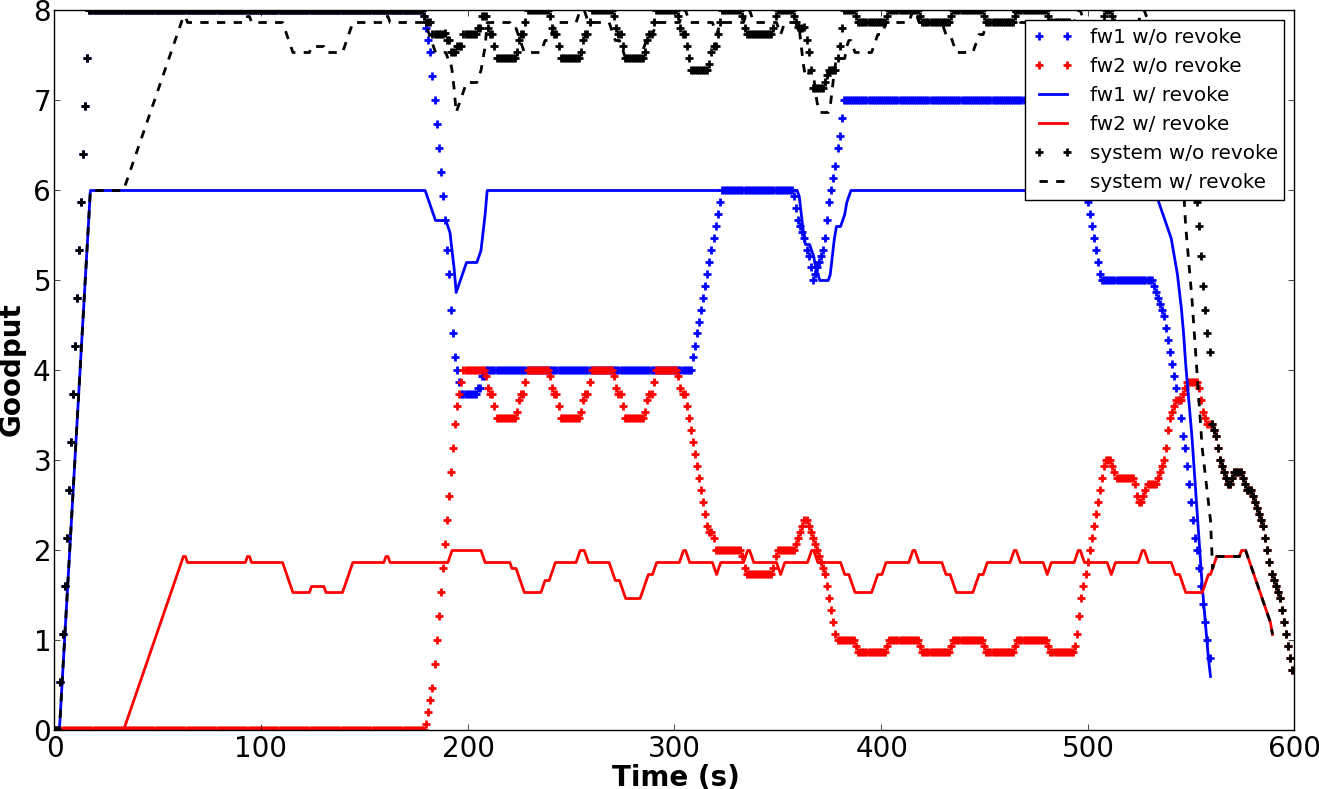
\includegraphics[width=\textwidth]{../results/30_goodput.png}
    \caption{Goodput Results for Scenario B}
    \label{fig:30-goodput}
  \end{subfigure}%
  \hfill
  \begin{subfigure}[t]{0.475\tw}\centering
    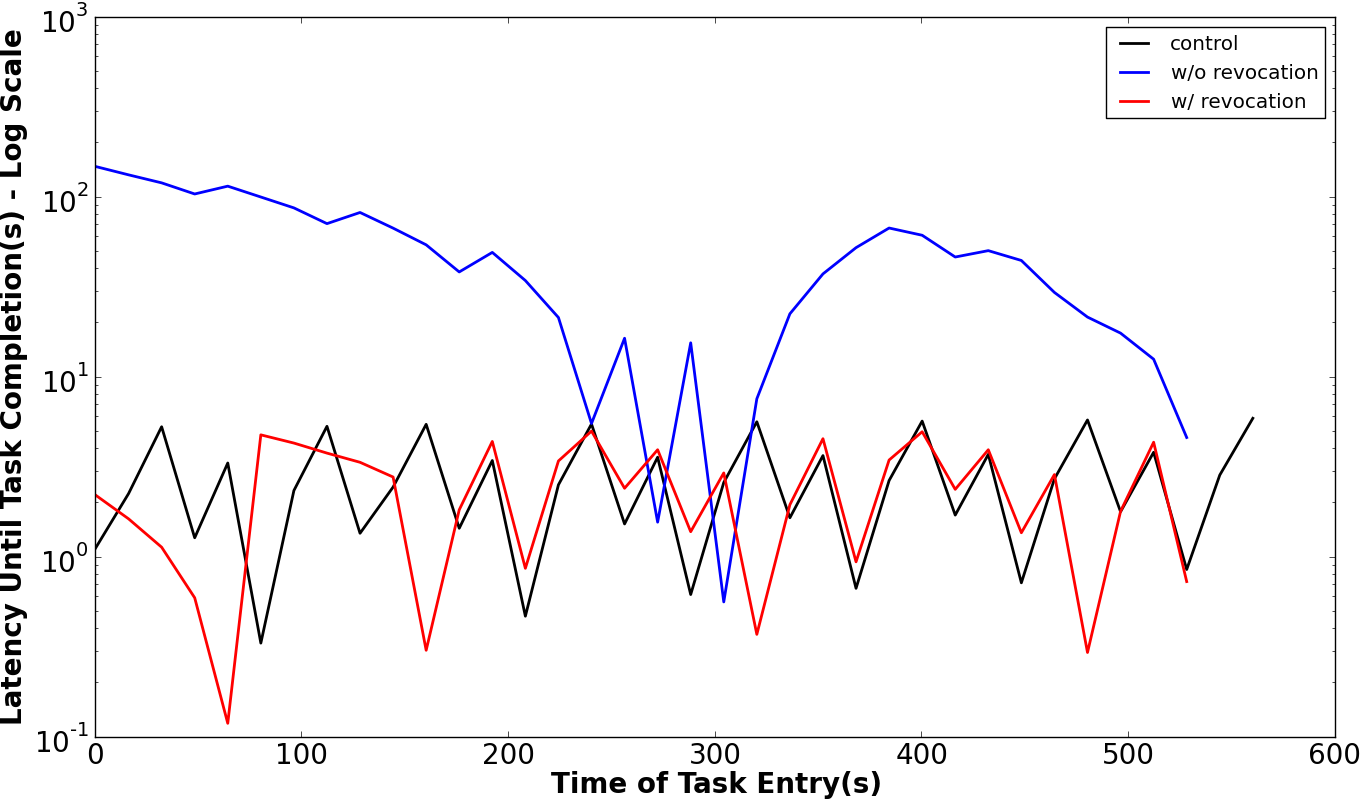
\includegraphics[width=\textwidth]{../results/30_fw_latency.png}
    \caption{Latency Results for Scenario B}
    \label{fig:30-latency}
  \end{subfigure}%

  \caption{\textbf{Goodput and Latency Results for Scenario B}
  Figure~\ref{fig:30-goodput} shows that there is still a fair amount of goodput loss in this scenario
  but the amount loss is much less than the amount in Scenario A. This is due to because the tasks
  that are killed have only made 30 seconds of progress whereas in Scenarios A the killed tasks have
  made 150 seconds of progress. Note that in this scenario, the second framework will experience
  a latency 2 orders of magnitude larger due to the fact, without resource revocation, they would have
  to wait even longer before they are given a slot in the system.
  }
  \label{fig:30-goodput-latency}
\end{figure*}
